%% For normal draft builds (figs undisplayed hence fast compile)
%\documentclass[hyperpdf,nobind,draft,oneside]{hepthesis}
%\documentclass[hyperpdf,nobind,draft,twoside]{hepthesis}

%% For short draft builds (breaks citations by necessity)
%documentclass[hyperpdf,nobind,draft,hidefrontback]{hepthesis}

%%For Cambridge soft-bound version
%\documentclass[hyperpdf,bindnopdf]{hepthesis}
%% For Cambridge hard-bound version (must be one-sided)
%\documentclass[hyperpdf,oneside]{hepthesis}
%%Get rid of warnings about list of figures and tables but also remove from ToC
\documentclass[hyperpdf,oneside,notlot,notlof]{hepthesis}

%% Load special font packages here if you wish
%\usepackage{lmodern}
%\usepackage{mathpazo}
%\usepackage{euler}

%% Put package includes etc. into preamble.tex for convenience
\usepackage{xspace}
\usepackage{tikz}
\usepackage{morefloats,subfig,afterpage}
\usepackage{mathrsfs} % script font
\usepackage{verbatim}
\usepackage{multirow}
\usepackage{nicematrix}
\usepackage{feynmf} % feynman diagrams

% glossary - add to toc and remove page numbers
\usepackage[xindy,toc,nonumberlist]{glossaries} 
%\newglossaryentry{domain-knowledge}{%
%  name={domain knowledge},%
%  description={valid knowledge used to refer to an area of human endeavour, an autonomous computer activity, or other specialized discipline}}

\newacronym{tla}{TLA}{Three Letter Acronym}
\newacronym{nist}{NIST}{National Institute of Standards and Technology}
\newacronym{larsoft}{LArSoft}{Liquid Argon Software}
\newacronym{sbn}{SBN}{Short Baseline Neutrino (Program)}
\newacronym{sbnd}{SBND}{Short Baseline Near Detector}
\newacronym{sce}{SCE}{Space Charge Effect}
\newacronym{sp}{SP}{Space Point}
\newacronym{argoneut}{ArgoNeuT}{Argon Neutrino Test Stand}
\newacronym{mc}{MC}{Monte Carlo}
\newacronym{mip}{MIP}{Minimum Ionising Particle}
\newacronym{adc}{ADC}{Analog Digital Converter}
\newacronym{tpc}{TPC}{Time Projection Chamber}
\newacronym{cpa}{CPA}{Cathode Plane Assembly}
\newacronym{apa}{APA}{Andode Plane Assembly}
\newacronym{pmt}{PMT}{Photo Multiplier Tube}
\newacronym{donut}{DONUT}{Direct Observation of the Nu Tau}
\newacronym{fermilab}{Fermilab}{Fermi National Accelerator Laboratory}
\newacronym{sm}{SM}{Standard Model}
\newacronym{sk}{SK}{Super Kamiokande}
\newacronym{sno}{SNO}{Sudbury Neutrino Observatory}
\newacronym{sage}{SAGE}{Soviet-American Gallium Experiment}
\newacronym{gallex}{GALLEX}{Gallium Experiment}
\newacronym{cc}{CC}{Charged Current}
\newacronym{ccqe}{CCQE}{Charged Current Quasi Elastic}
\newacronym{nc}{NC}{Neutral Current}
\newacronym{es}{ES}{Elastic Scattering}
\newacronym{pmns}{PMNS}{Pontecorvo-Maki-Nakagawa-Sakata}
\newacronym{cp}{CP}{Charge-Parity}
\newacronym{pdg}{PDG}{Particle Data Group}
\newacronym{karmen}{KARMEN}{Karlsruhe Rutherford Medium Energy Neutrino}
\newacronym{minos}{MINOS}{Main Injector Neutrino Oscillation Search}
\newacronym{lsnd}{LSND}{Liquid Scintillator Neutrino Detector}
\newacronym{miniboone}{MiniBooNE}{Mini Booster Neutrino Experiment}
\newacronym{microboone}{MicroBooNE}{Micro Booster Neutrino Experiment}
\newacronym{bnb}{BNB}{Booster Neutrino Beam}




%\makeglossaries

%% Using Babel allows other languages to be used and mixed-in easily
%\usepackage[ngerman,english]{babel}
\usepackage[english]{babel}
\selectlanguage{english}

%% Citation system tweaks
\usepackage{cite}
% \let\@OldCite\cite
% \renewcommand{\cite}[1]{\mbox{\!\!\!\@OldCite{#1}}}

%\usepackage{titlesec}

%% Maths
% TODO: rework or eliminate maybemath
\usepackage{abmath}
\DeclareRobustCommand{\mymath}[1]{\ensuremath{\maybebmsf{#1}}}
% \DeclareRobustCommand{\parenths}[1]{\mymath{\left({#1}\right)}\xspace}
% \DeclareRobustCommand{\braces}[1]{\mymath{\left\{{#1}\right\}}\xspace}
% \DeclareRobustCommand{\angles}[1]{\mymath{\left\langle{#1}\right\rangle}\xspace}
% \DeclareRobustCommand{\sqbracs}[1]{\mymath{\left[{#1}\right]}\xspace}
% \DeclareRobustCommand{\mods}[1]{\mymath{\left\lvert{#1}\right\rvert}\xspace}
% \DeclareRobustCommand{\modsq}[1]{\mymath{\mods{#1}^2}\xspace}
% \DeclareRobustCommand{\dblmods}[1]{\mymath{\left\lVert{#1}\right\rVert}\xspace}
% \DeclareRobustCommand{\expOf}[1]{\mymath{\exp{\!\parenths{#1}}}\xspace}
% \DeclareRobustCommand{\eexp}[1]{\mymath{e^{#1}}\xspace}
% \DeclareRobustCommand{\plusquad}{\mymath{\oplus}\xspace}
% \DeclareRobustCommand{\logOf}[1]{\mymath{\log\!\parenths{#1}}\xspace}
% \DeclareRobustCommand{\lnOf}[1]{\mymath{\ln\!\parenths{#1}}\xspace}
% \DeclareRobustCommand{\ofOrder}[1]{\mymath{\mathcal{O}\parenths{#1}}\xspace}
% \DeclareRobustCommand{\SOgroup}[1]{\mymath{\mathup{SO}\parenths{#1}}\xspace}
% \DeclareRobustCommand{\SUgroup}[1]{\mymath{\mathup{SU}\parenths{#1}}\xspace}
% \DeclareRobustCommand{\Ugroup}[1]{\mymath{\mathup{U}\parenths{#1}}\xspace}
% \DeclareRobustCommand{\I}[1]{\mymath{\mathrm{i}}\xspace}
% \DeclareRobustCommand{\colvector}[1]{\mymath{\begin{pmatrix}#1\end{pmatrix}}\xspace}
\DeclareRobustCommand{\Rate}{\mymath{\Gamma}\xspace}
\DeclareRobustCommand{\RateOf}[1]{\mymath{\Gamma}\parenths{#1}\xspace}

%% High-energy physics stuff
\usepackage{abhep}
\usepackage{hepnames}
\usepackage{hepunits}
\DeclareRobustCommand{\arXivCode}[1]{arXiv:#1}
\DeclareRobustCommand{\CP}{\ensuremath{\mathcal{CP}}\xspace}
\DeclareRobustCommand{\CPviolation}{\CP-violation\xspace}
\DeclareRobustCommand{\CPv}{\CPviolation}
\DeclareRobustCommand{\LHCb}{LHCb\xspace}
\DeclareRobustCommand{\LHC}{LHC\xspace}
\DeclareRobustCommand{\LEP}{LEP\xspace}
\DeclareRobustCommand{\CERN}{CERN\xspace}
\DeclareRobustCommand{\bphysics}{\Pbottom-physics\xspace}
\DeclareRobustCommand{\bhadron}{\Pbottom-hadron\xspace}
\DeclareRobustCommand{\Bmeson}{\PB-meson\xspace}
\DeclareRobustCommand{\bbaryon}{\Pbottom-baryon\xspace}
\DeclareRobustCommand{\Bdecay}{\PB-decay\xspace}
\DeclareRobustCommand{\bdecay}{\Pbottom-decay\xspace}
\DeclareRobustCommand{\BToKPi}{\HepProcess{ \PB \to \PK \Ppi }\xspace}
\DeclareRobustCommand{\BToPiPi}{\HepProcess{ \PB \to \Ppi \Ppi }\xspace}
\DeclareRobustCommand{\BToKK}{\HepProcess{ \PB \to \PK \PK }\xspace}
\DeclareRobustCommand{\BToRhoPi}{\HepProcess{ \PB \to \Prho \Ppi }\xspace}
\DeclareRobustCommand{\BToRhoRho}{\HepProcess{ \PB \to \Prho \Prho }\xspace}
\DeclareRobustCommand{\X}{\thesismath{X}\xspace}
\DeclareRobustCommand{\Xbar}{\thesismath{\overline{X}}\xspace}
\DeclareRobustCommand{\Xzero}{\HepGenParticle{X}{}{0}\xspace}
\DeclareRobustCommand{\Xzerobar}{\HepGenAntiParticle{X}{}{0}\xspace}
\DeclareRobustCommand{\epluseminus}{\Ppositron\!\Pelectron\xspace}
\DeclareRobustCommand{\protonproton}{\Pproton\APantiproton\xspace}


%% You can set the line spacing this way
%\setallspacing{double}
%% or a section at a time like this
%\setfrontmatterspacing{double}


%% Define the thesis title and author
\title{Energy Reconstruction Tech Note}
\author{All the authors..}

%% Doc-specific PDF metadata
\makeatletter
\@ifpackageloaded{hyperref}{%
\hypersetup{%
  pdftitle = {Search for Sterile Neutrinos at the SBN program},
  pdfsubject = {Andy Buckley's PhD thesis},
  pdfkeywords = {LHCb, B, physics, LHC, heavy flavour},
  pdfauthor = {}
}}{}
\makeatother

% Redeclare the \EquationRef command so it uses \ref instead of \eqnref
\DeclareRobustCommand{\EquationRef}{Equation \ref}

%\titleformat{\chapter}[display]
%  {\normalfont\bfseries}{}{0pt}{\Huge}
%\titlespacing*{\chapter}
%  {0pt}{20pt}{40pt}

%% Start the document
\begin{document}

%% Define the un-numbered front matter (cover pages, rubrik and table of contents)
\begin{frontmatter}
  %% Title
\titlepage[\ ]{%
  Some more stuff}

%% Acknowledgements
%\begin{acknowledgements}
%  Acknowledgements\dots
%\end{acknowledgements}

%% Abstract
%\begin{abstract}%[\smaller \thetitle\\ \vspace*{1cm} \smaller {\theauthor}]
  %\thispagestyle{empty}
%  Abstract..
%\end{abstract}


%% Declaration
%\begin{declaration}
%  Declaration
%  \vspace*{1cm}
%  \begin{flushright}
%    Name??
%  \end{flushright}
%\end{declaration}





%% Preface
%\begin{preface}
%  Preface??
%\end{preface}

%% ToC
\tableofcontents


%% Strictly optional!
%\frontquote{%
%  Writing in English is the most ingenious torture\\
%  ever devised for sins committed in previous lives.}%
%  {James Joyce}
%% I don't want a page number on the following blank page either.
\thispagestyle{empty}

%% Add Glossary
%\glsaddall 
%\printglossaries

%% I prefer to put these tables here rather than making the
%% front matter seemingly interminable. No-one cares, anyway!
%\listoffigures
%\listoftables






\end{frontmatter}

%% Start the content body of the thesis
\begin{mainmatter}
  %% Actually, more semantic chapter filenames are better, like "chap-bgtheory.tex"
  \chapter{Introduction}
\label{chap:Introduction}
%% Restart the numbering to make sure that this is definitely page #1!
\pagenumbering{arabic}


  \chapter{Motivation}
\label{chap:Motivation}

\begin{itemize}
    \item Where reco. energy is used and why it's needed? (nue selection etc)
    \item Why ESTAR method is better motivated than other methods?
    \item Need a nice way to correct for SCE - explain SCE here? 
\end{itemize}
  \chapter{Method}
\label{chap:Method}

\begin{itemize}
    \item Explanation of larsoft/Pandora - don't really know..
    \item Explain ESTAR method \cite{ESTAR_Database}
    \item Compare/reference previous methods too? 
\end{itemize}

\section{Overview}

\textcolor{red}{ADDITIONAL DETAIL ON EARLIER STEPS??}

To estimate the reconstructed shower energy, the hits from the shower are found and integrated over to obtain the collected charge in \Gls{adc} units. This is then converted to a conventional charge (number of electrons) by a calibration factor. The reconstruction is done on a per-hit basis which means that any corrections are done for each individual hit and the reconstructed energy of each hit is calculated. The total shower energy is then found by summing up the energy of all associated hits. 

Detector effects such as electron lifetime and recombination must also be considered. The drifting electrons have a finite lifetime in the detector because they will eventually attach to positively charged impurities in the argon \cite{ArgoNeuT_electron_lifetime_paper}. Due to this, the collected charge has to be corrected to account for the electron lifetime. The other effect to consider is electron recombination. When argon atoms are ionised, the resulting argon ion and ionised electron may immediately recombine. This is known as the recombination effect and the magnitude of the effect is largely due to the local electric field \cite{ArgoNeuT_recombination_paper}. The recombination effect is modelled by the Modified Box recombination model and is given by
\begin{equation}\label{eqn:ModBox}
    \frac{dE}{dx} = \frac{\exp{(\frac{\beta}{\rho \mathcal{E}} W_{ion}.\frac{dQ}{dx}}) - \alpha}{\frac{\beta}{\rho \mathcal{E}}},
\end{equation}
where $\frac{dE}{dx}$ is the deposited energy per unit length, $\frac{dQ}{dx}$ is the deposited charge per unit length,  $\mathcal{E}$ is the electric field in the detector, $\rho$ is the density of liquid argon, $W_{ion} = 23.6$ eV which is the energy required to ionise an argon atom, $\alpha = 0.93 \pm 0.02$ and $\beta = 0.212 \pm 0.002$ (kV/cm)(g/cm$^2$)/MeV. The values for parameters $\alpha$ and $\beta$ are results from the \Gls{argoneut} experiment \cite{ArgoNeuT_recombination_paper}.

To convert the collected charge to energy, we will use the Modified Box recombination model in conjunction with the ESTAR database. The ESTAR database is provided by the \Gls{nist} and gives the track length of electrons in liquid argon for energies ranging from 0.01 MeV to 1000 MeV \cite{ESTAR_Database}. This allows $\frac{dE}{dx}$ values to be calculated by dividing the energy by the track length for each entry in the ESTAR database. The deposited charge, Q, is then found by using \EquationRef{eqn:ModBox} to find $\frac{dQ}{dx}$ and multiplying by the track length, \textit{dx}. This now allows the deposited charge and energy to be related. If $\mathcal{E}$ in \EquationRef{eqn:ModBox} is taken to be a variable, the above process is repeated whilst iterating over set values of $\mathcal{E}$. This results in a 3D curve relating both the deposited charge and electric field to energy as is shown in \FigureRef{fig:ESTAR lookup curve}. The energy is interpolated from the deposited charge and electric field. A direct recombination correction is not required with this method as it has already been accounted for in the lookup curve. 

\begin{figure}[h]
    \centering
    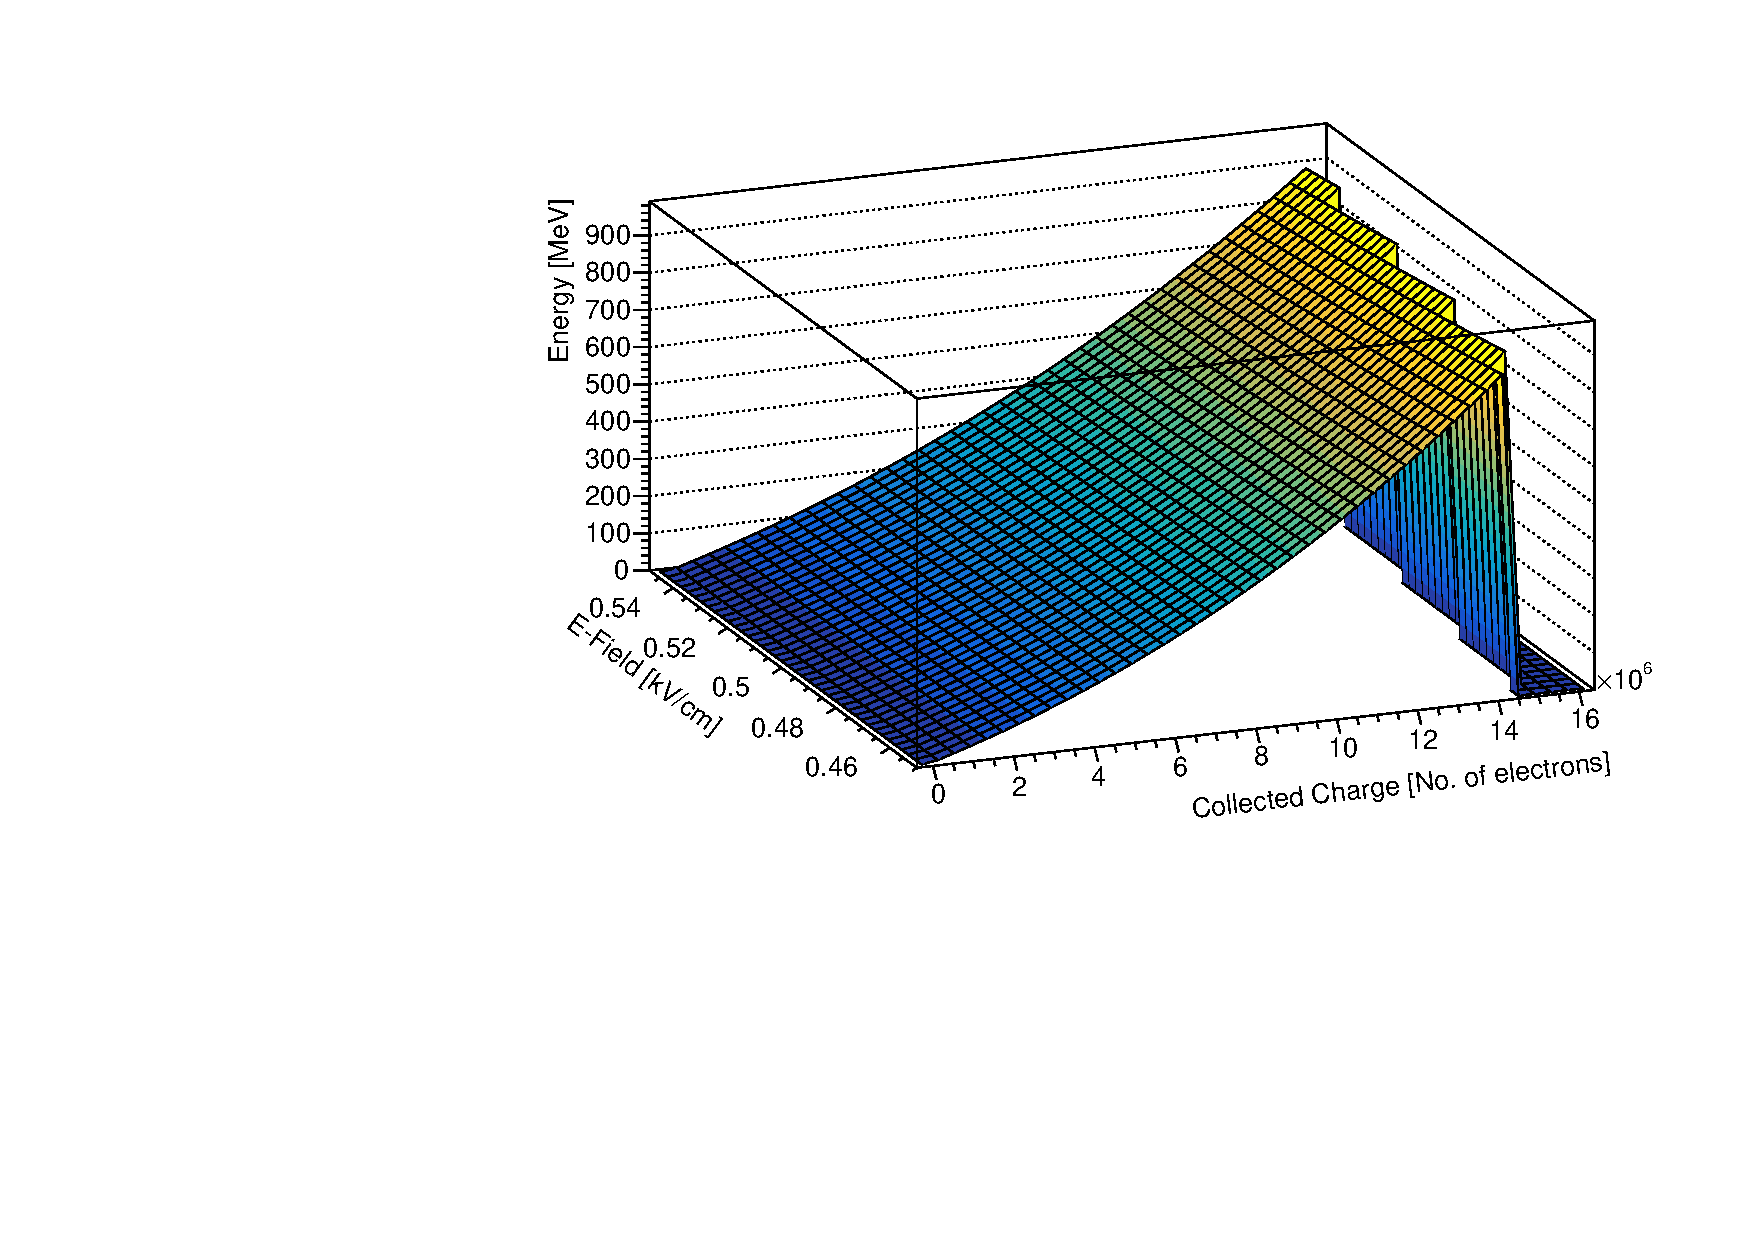
\includegraphics[width = \largefigwidth]{Figures/ESTAR_lookup_curve.pdf}
    \caption{The collected energy as a function of the collected charge and the local electric field. Produced with data from the ESTAR database and use of the Modified Box recombination model.}
    \label{fig:ESTAR lookup curve}
\end{figure}

\newpage
\section{Correcting for SCE}
Since the \gls{sce} causes the electric field in the detector to be non-uniform, the local electric field at each point in the detector needs to be known. An example map of the electric field in the centre of \gls{sbnd} is shown in \FigureRef{fig:SCE map}. To account for each hit being associated with a different value of the electric field, the corresponding \Glspl{sp} for each of the hits are found and the coordinates of the \glspl{sp} in the detector are determined. Instead of using the nominal value for $\mathcal{E}$, the local value for $\mathcal{E}$ at the position of the \Glspl{sp} is used when interpolating the energy. In the case that a hit has no corresponding \Glspl{sp}, the charge weighted centre of the shower is found and the local value of $\mathcal{E}$ at this point is used instead. The charge weighted centre is defined as $\frac{\sum (charge \times position)}{\sum charge}$ from the available \glspl{sp}.

\begin{figure}[h]
    \centering
    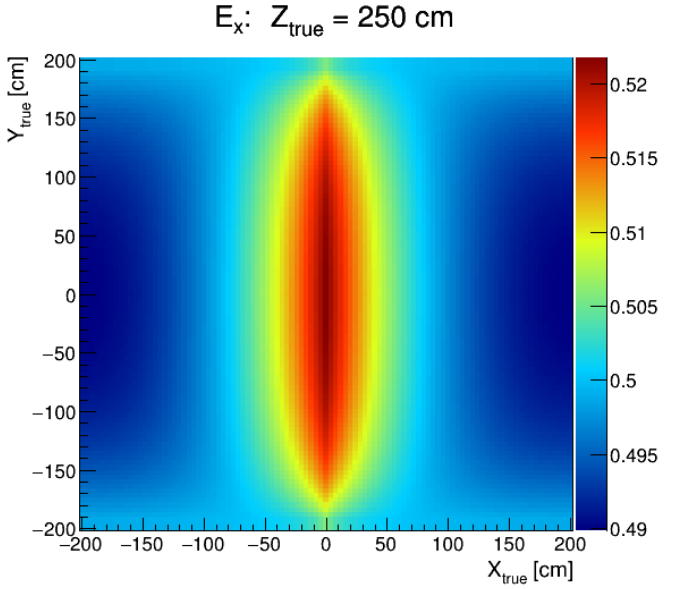
\includegraphics[width = \largefigwidth]{Figures/SCE_map_SBND.png}
    \caption{The expected electric field offset relative to the nominal value of 0.5 kV/cm at z = 250cm in SBND (the centre of the detector) caused by SCE.}
    \label{fig:SCE map}
\end{figure}


















  \chapter{Validation}
\label{chap:Validation}

Samples:
\begin{itemize}
    \item \textcolor{green}{Standard BNB $\electron \pi^+$}
    \item \textcolor{green}{Standard BNB $\gamma \pi^+$}
    \item \textcolor{green}{Standard BNB cheating $\electron \pi^+$}
    \item \textcolor{orange}{SCE cheating cathode BNB $\electron \pi^+$}
    \item \textcolor{orange}{SCE cheating anode BNB $\electron \pi^+$}
    \item \textcolor{green}{XZ plane cheating $\electron \pi^+$ - may need to remake with uniform angular dist.}
    \item \textcolor{green}{YZ plane cheating $\electron \pi^+$}
    \item \textcolor{red}{Standard BNB with lower thresholding $\electron \pi^+$}
    \item \textcolor{red}{Some low energy sample}
\end{itemize}

\begin{figure}
    \centering
    \fbox{Fractional resolution using $\electron \pi^+$ BNB vertex sample for plane 0}
    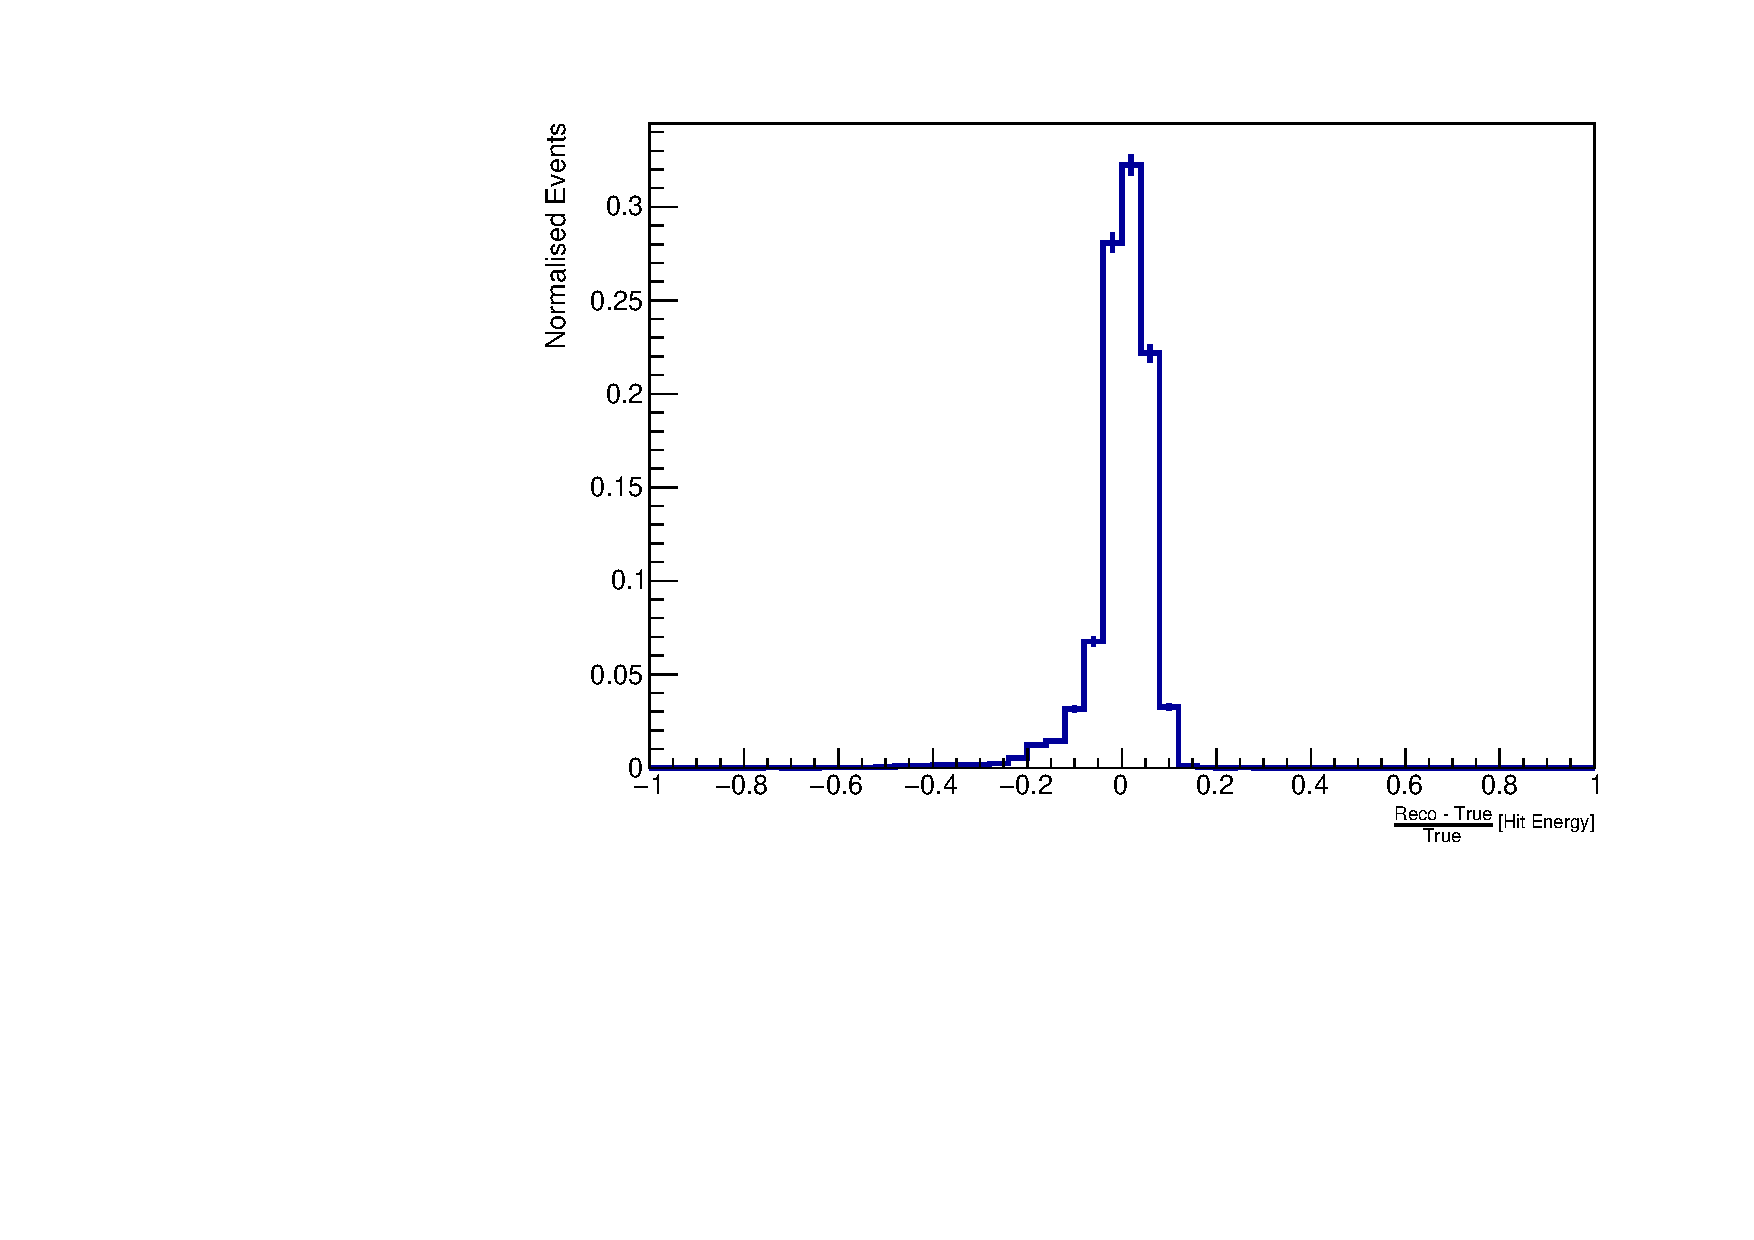
\includegraphics[width = \largefigwidth]{Figures/fractional_res_standard_electron_vertex_plane0.pdf}
    \caption{Fractional resolution of the shower energy from an $\electron \pi^+$ vertex sample. Reconstruction performed from the hits collected by plane 0.}
    \label{fig:my_label}
\end{figure}

\begin{figure}
    \centering
    \fbox{Fractional resolution using $\electron \pi^+$ BNB vertex sample for plane 1}
    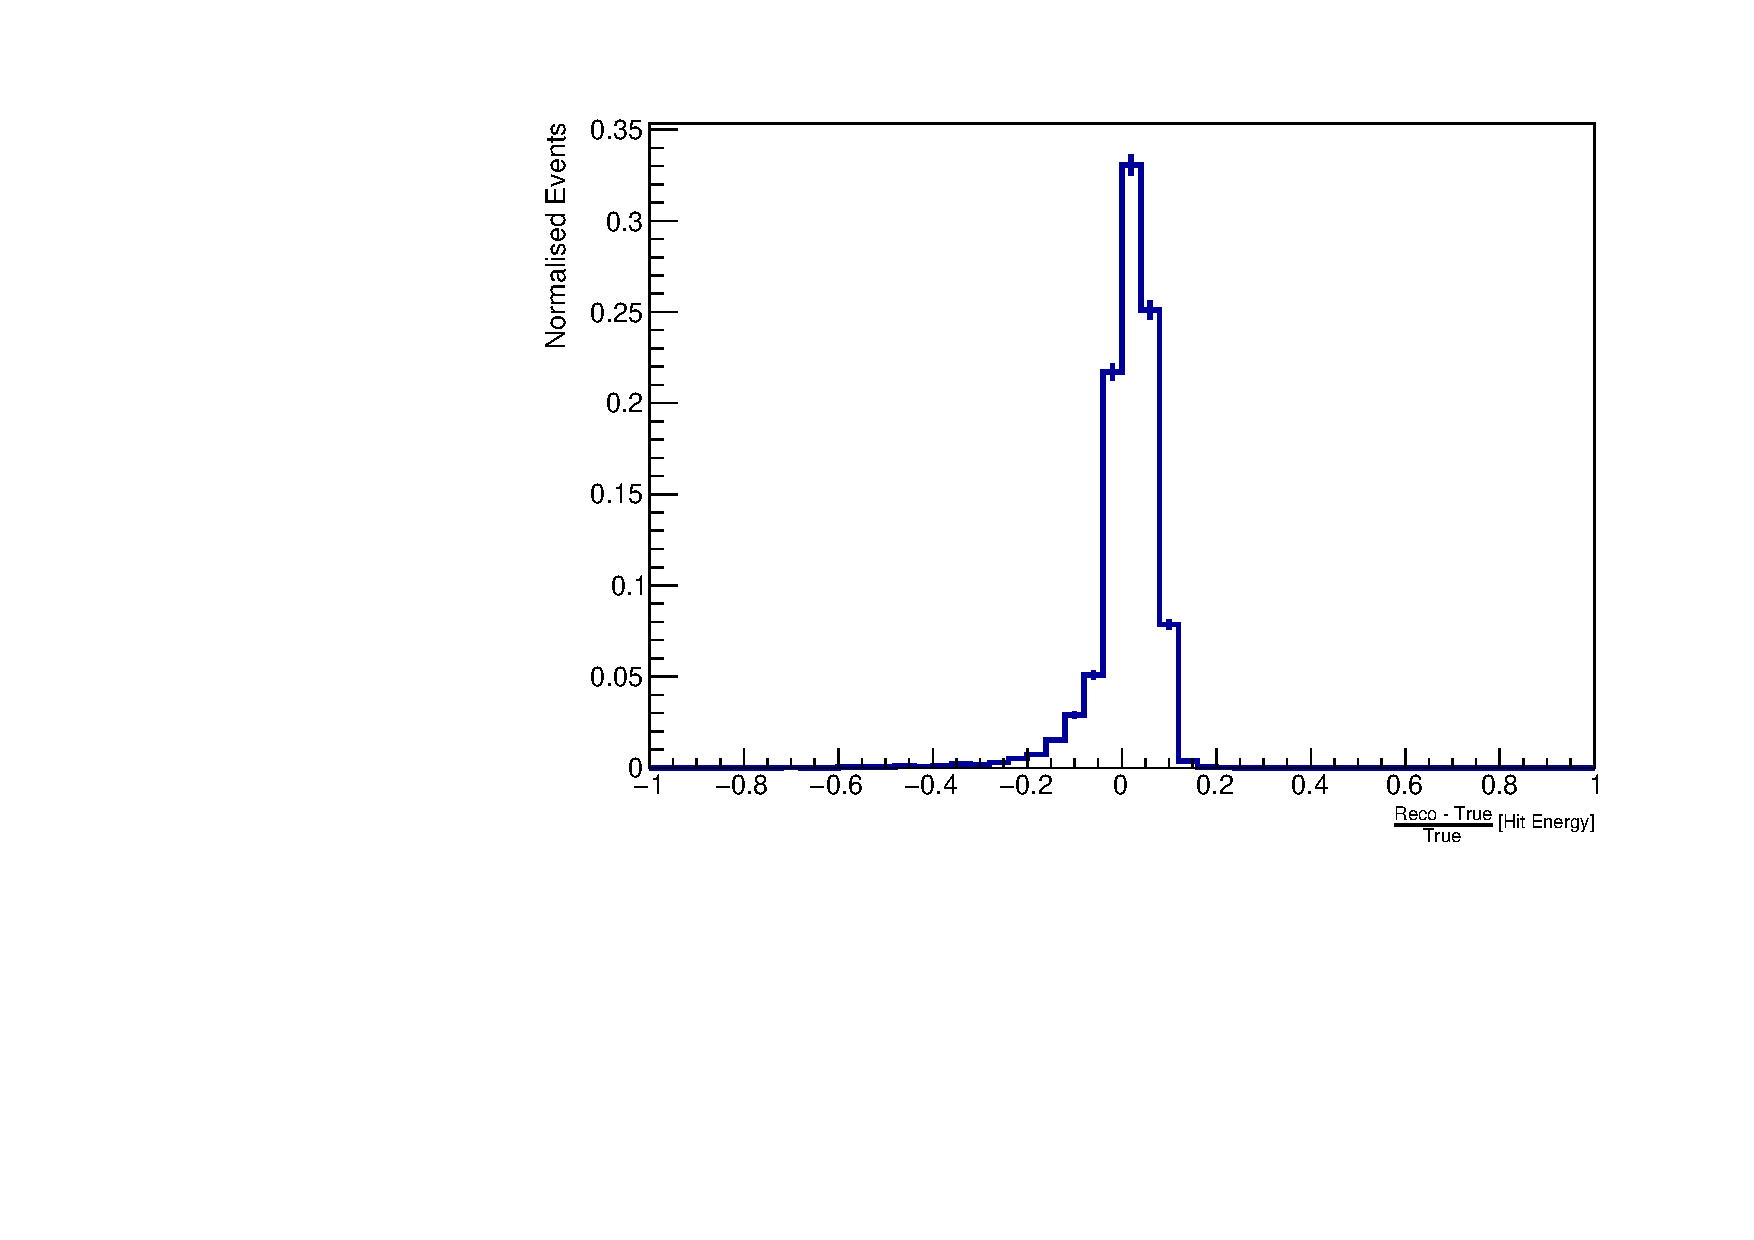
\includegraphics[width = \largefigwidth]{Figures/fractional_res_standard_electron_vertex_plane1.pdf}
    \caption{Fractional resolution of the shower energy from an $\electron \pi^+$ vertex sample. Reconstruction performed from the hits collected by plane 1.}
    \label{fig:my_label}
\end{figure}

\begin{figure}
    \centering
    \fbox{Fractional resolution using $\electron \pi^+$ BNB vertex sample for plane 2}
    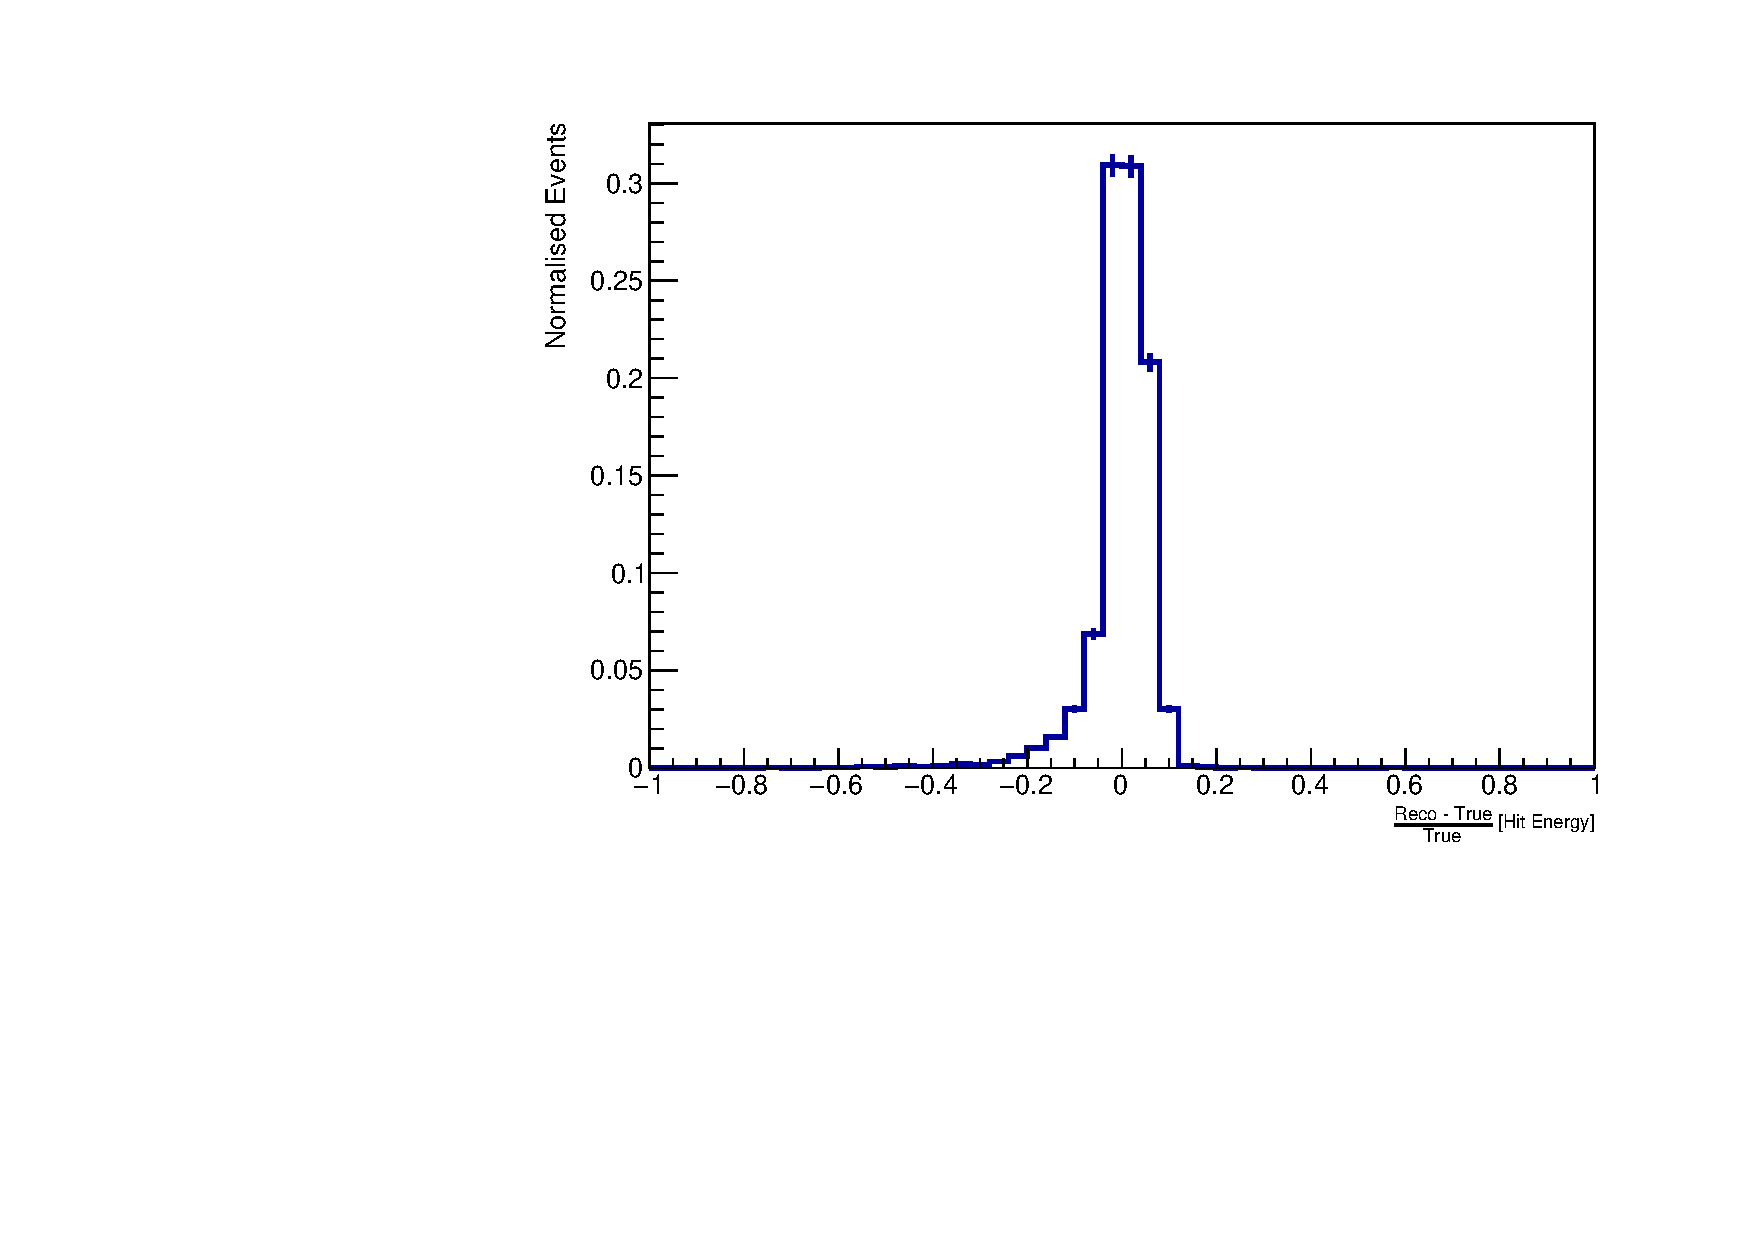
\includegraphics[width = \largefigwidth]{Figures/fractional_res_standard_electron_vertex_plane2.pdf}
    \caption{Fractional resolution of the shower energy from an $\electron \pi^+$ vertex sample. Reconstruction performed from the hits collected by plane 2.}
    \label{fig:my_label}
\end{figure}

\begin{figure}
    \centering
    \fbox{Fractional resolution using $\electron \pi^+$ BNB vertex sample for the best plane}
    \caption{Fractional resolution of the shower energy from an $\electron \pi^+$ vertex sample. Reconstruction performed from the hits collected by the \textit{best} plane which is defined as the plane with the most hits.}
    \label{fig:my_label}
\end{figure}

\begin{figure}
    \centering
    \fbox{Fractional resolution using $\electron \pi^+$ BNB vertex sample with cheated pattern recognition.}
    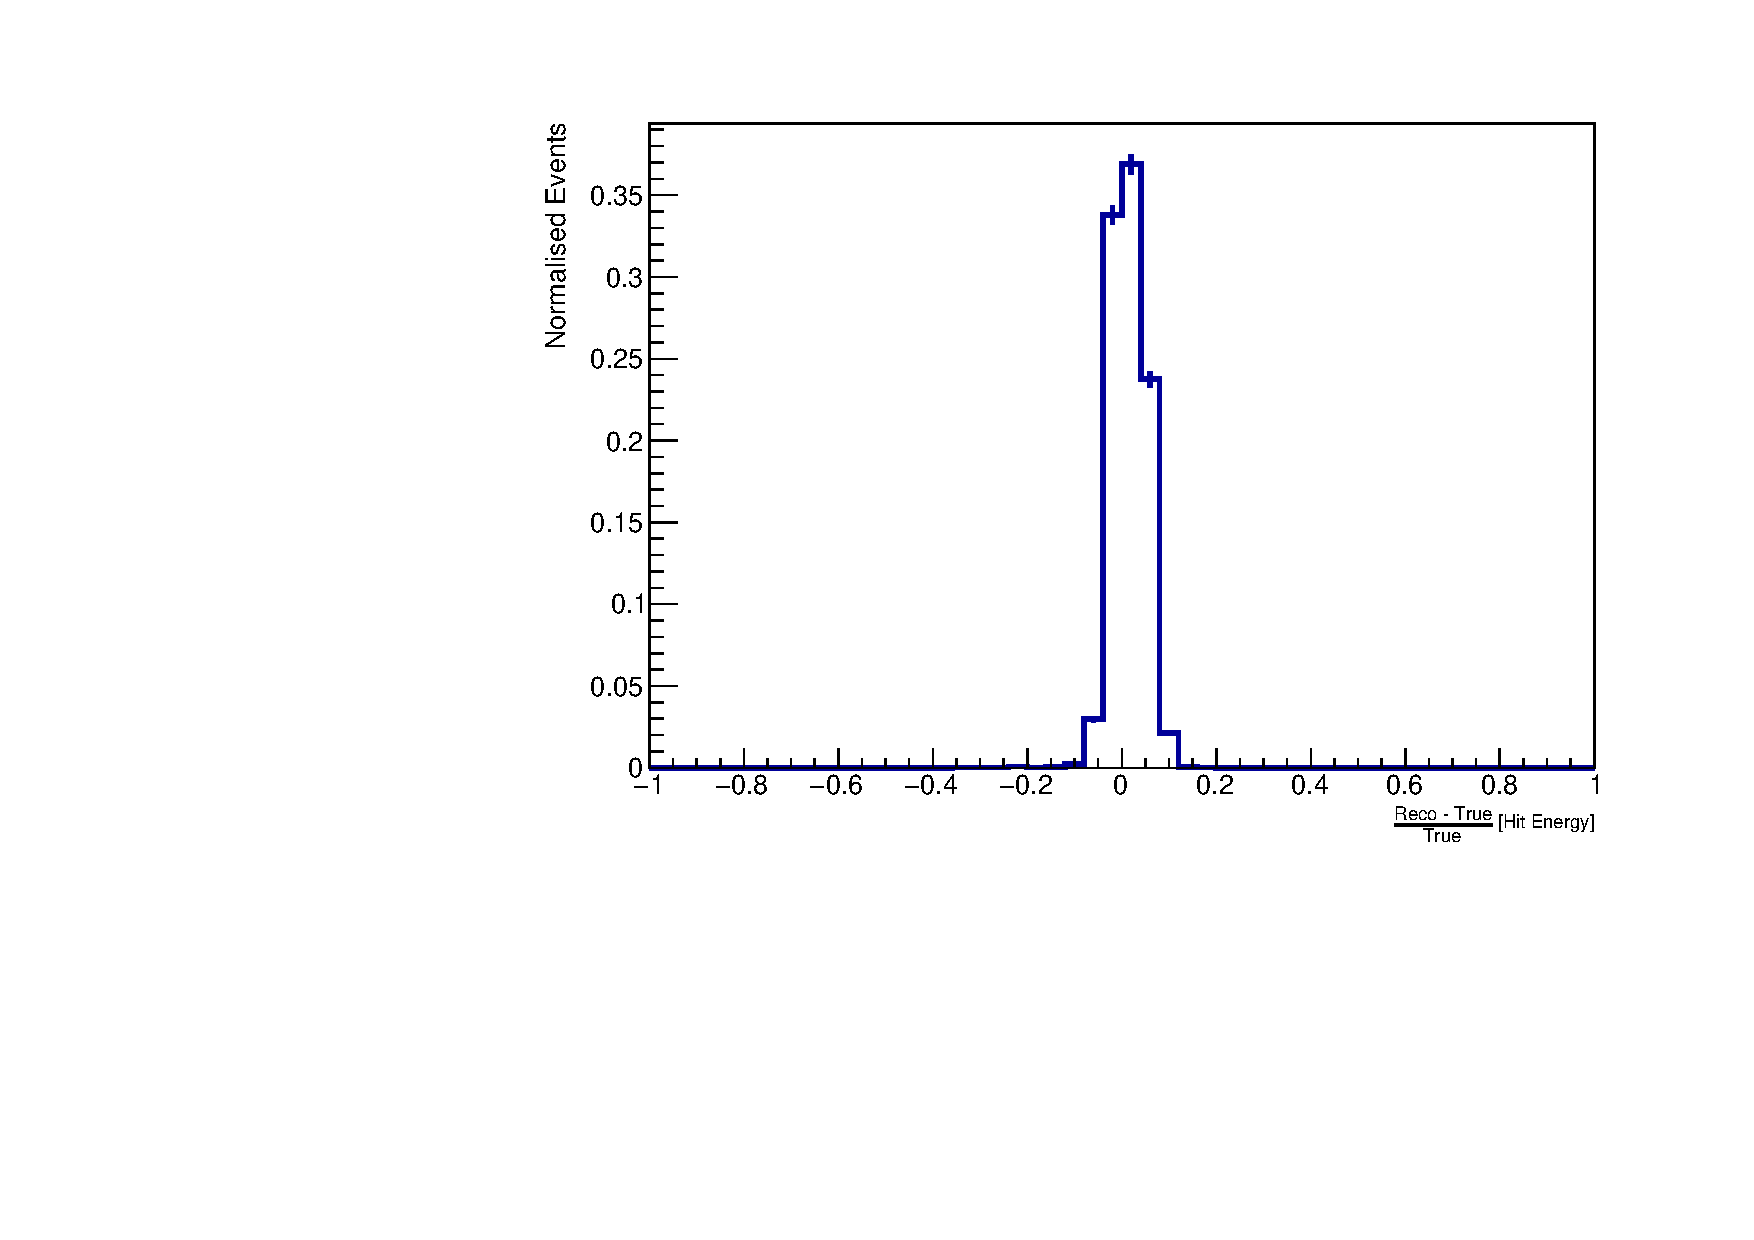
\includegraphics[width = \largefigwidth]{Figures/fractional_res_standard_cheating_electron_vertex_plane2.pdf}
    \caption{Fractional resolution of the shower energy from an $\electron \pi^+$ vertex sample with cheated pattern recognition. Reconstruction performed from the hits collected by plane 2.}
    \label{fig:my_label}
\end{figure}

\begin{figure}
    \centering
    \fbox{Fractional resolution using $\gamma \pi^+$ BNB vertex sample}
    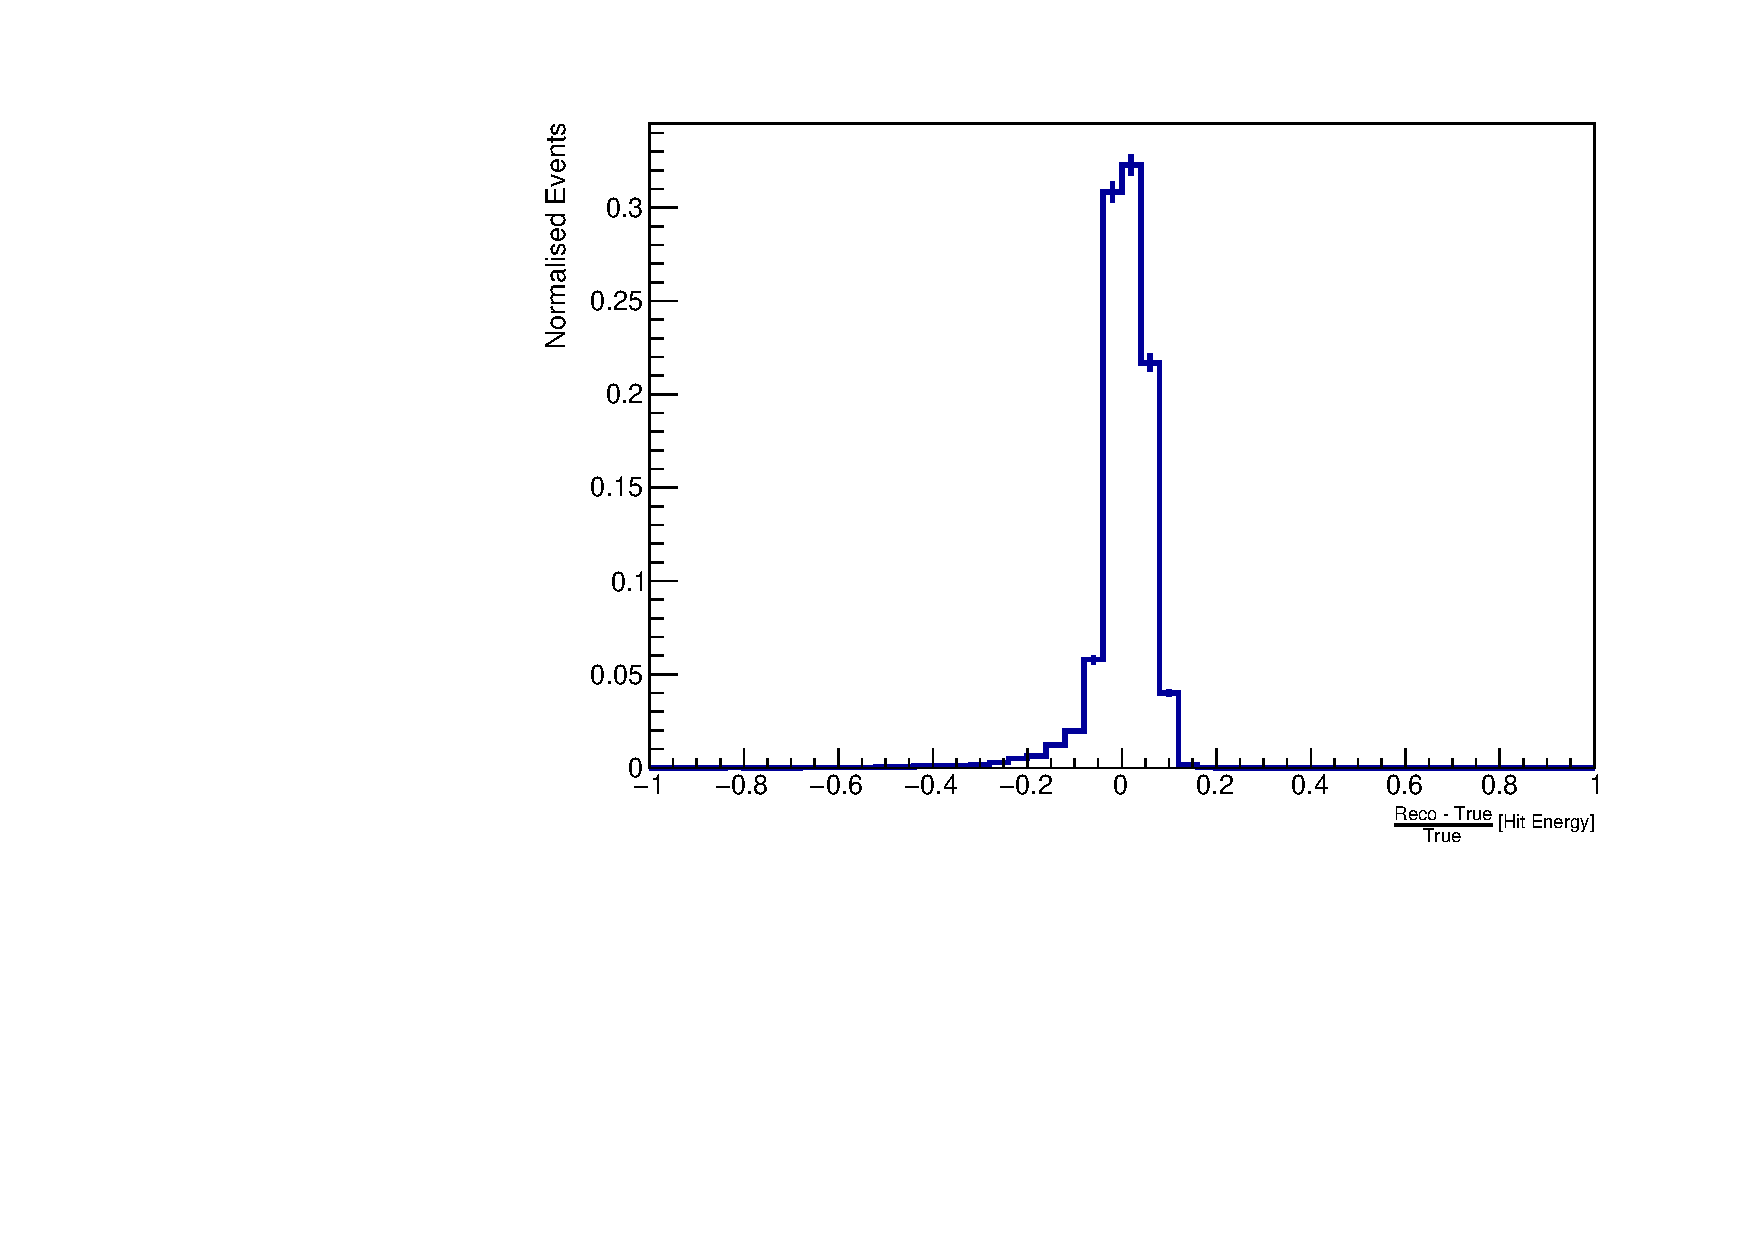
\includegraphics[width = \largefigwidth]{Figures/fractional_res_standard_gamma_vertex_plane2.pdf}
    \caption{Fractional resolution of the shower energy using a $\gamma \pi^+$ vertex sample. Reconstruction performed from the hits collected by plane 2.}
    \label{fig:my_label}
\end{figure}

\begin{figure}
    \centering
    \fbox{
    \begin{minipage}{0.8\textwidth}
    Space Charge validation. Fractional resolution plot for cathode sample w.o. SCE, w. SCE but no correction and w. SCE + correction. Plus include ratio plot.
    Use cheated pattern recognition. \newline
    
    \end{minipage}
    }
    \caption{Caption}
    \label{fig:my_label}
\end{figure}

\begin{figure}
    \centering
    \fbox{
    \begin{minipage}{0.8\textwidth}
    Space Charge validation. Fractional resolution plot for anode sample w.o. SCE, w. SCE but no correction and w. SCE + correction. Plus include ratio plot.
    Use cheated pattern recognition. \newline
    
    \end{minipage}
    }
    \caption{Caption}
    \label{fig:my_label}
\end{figure}













  \chapter{Additional Studies}
\label{chap:Additional Studies}

\begin{figure}
    \centering
    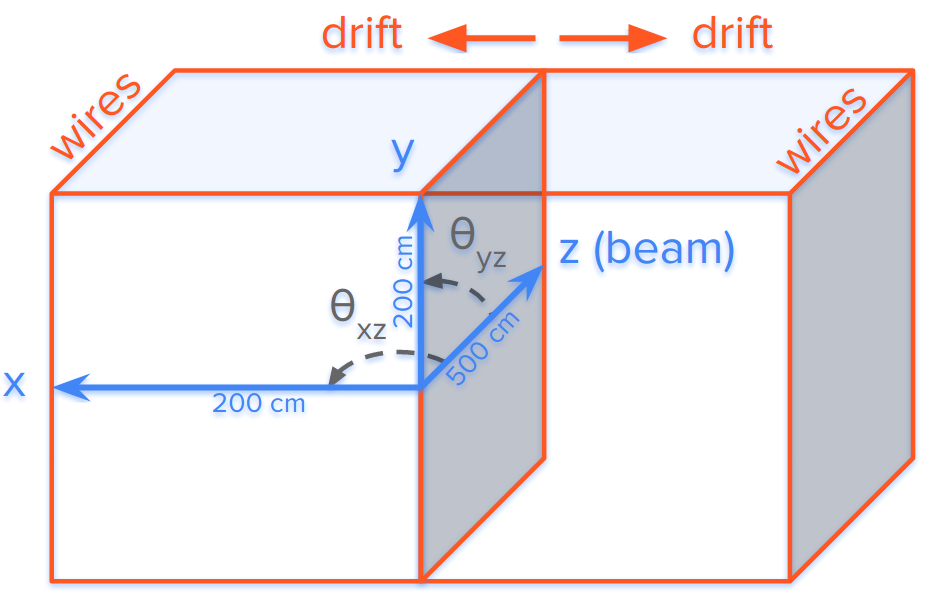
\includegraphics[width =\largefigwidth]{Figures/SBND_geometry.png}
    \caption{The SBND coordinate system showing the definition of the $\theta_{XZ}$ and $\theta_{YZ}$ angles.}
    \label{fig:my_label}
\end{figure}

Expect the hit resolution to be poor when showers are directed in the drift direction. There will be a large pulse train on just a few wires which means the hit reconstruction will suffer. 
\begin{figure}
    \centering
    \fbox{
    \begin{minipage}{0.8\textwidth}
    Reco efficiency vs XZ angle (Y is fixed at 0m).
    Don't think I understand why there is a local peak at +- 90ish degrees, I would have expected the performance to be at its worst for these cases. Otherwise looks sensible I think. 
    \end{minipage}
    }
    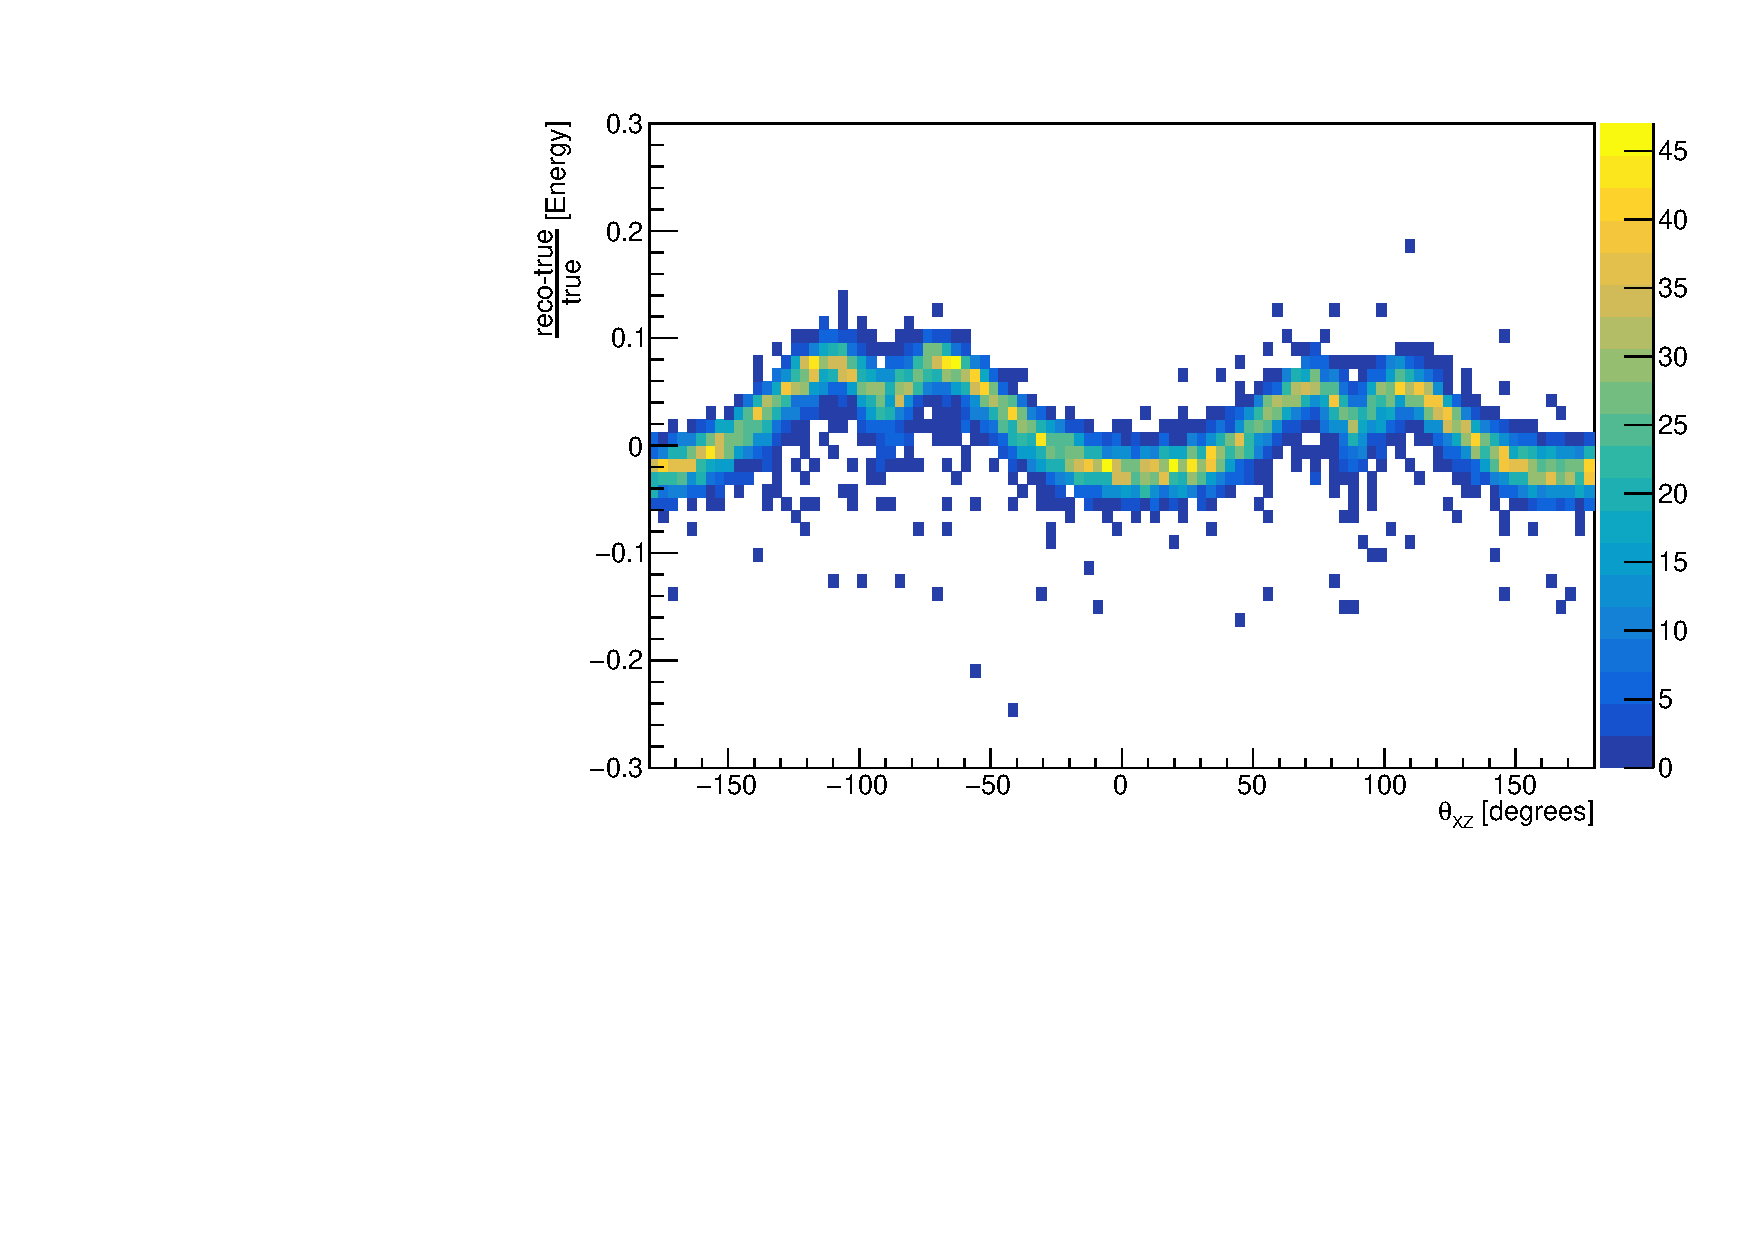
\includegraphics[width = \largefigwidth]{Figures/frac_res_vs_thetaXZ_cheating_electron_vertex_plane2.pdf}
    \caption{The fractional resolution of the shower energy from an $\electron \pi^+$ vertex sample vs the angle of the electron in the X-Z plane (i.e. Y is fixed at 0). Reconstruction performed from the hits collected by plane 2.}
    \label{fig:my_label}
\end{figure}

\begin{figure}
    \centering
    \fbox{Reco efficiency vs YZ angle (X is fixed at 1m)}
    \caption{Caption}
    \label{fig:my_label}
\end{figure}

\begin{figure}
    \centering
    \fbox{Reco efficiency vs true deposited energy}
    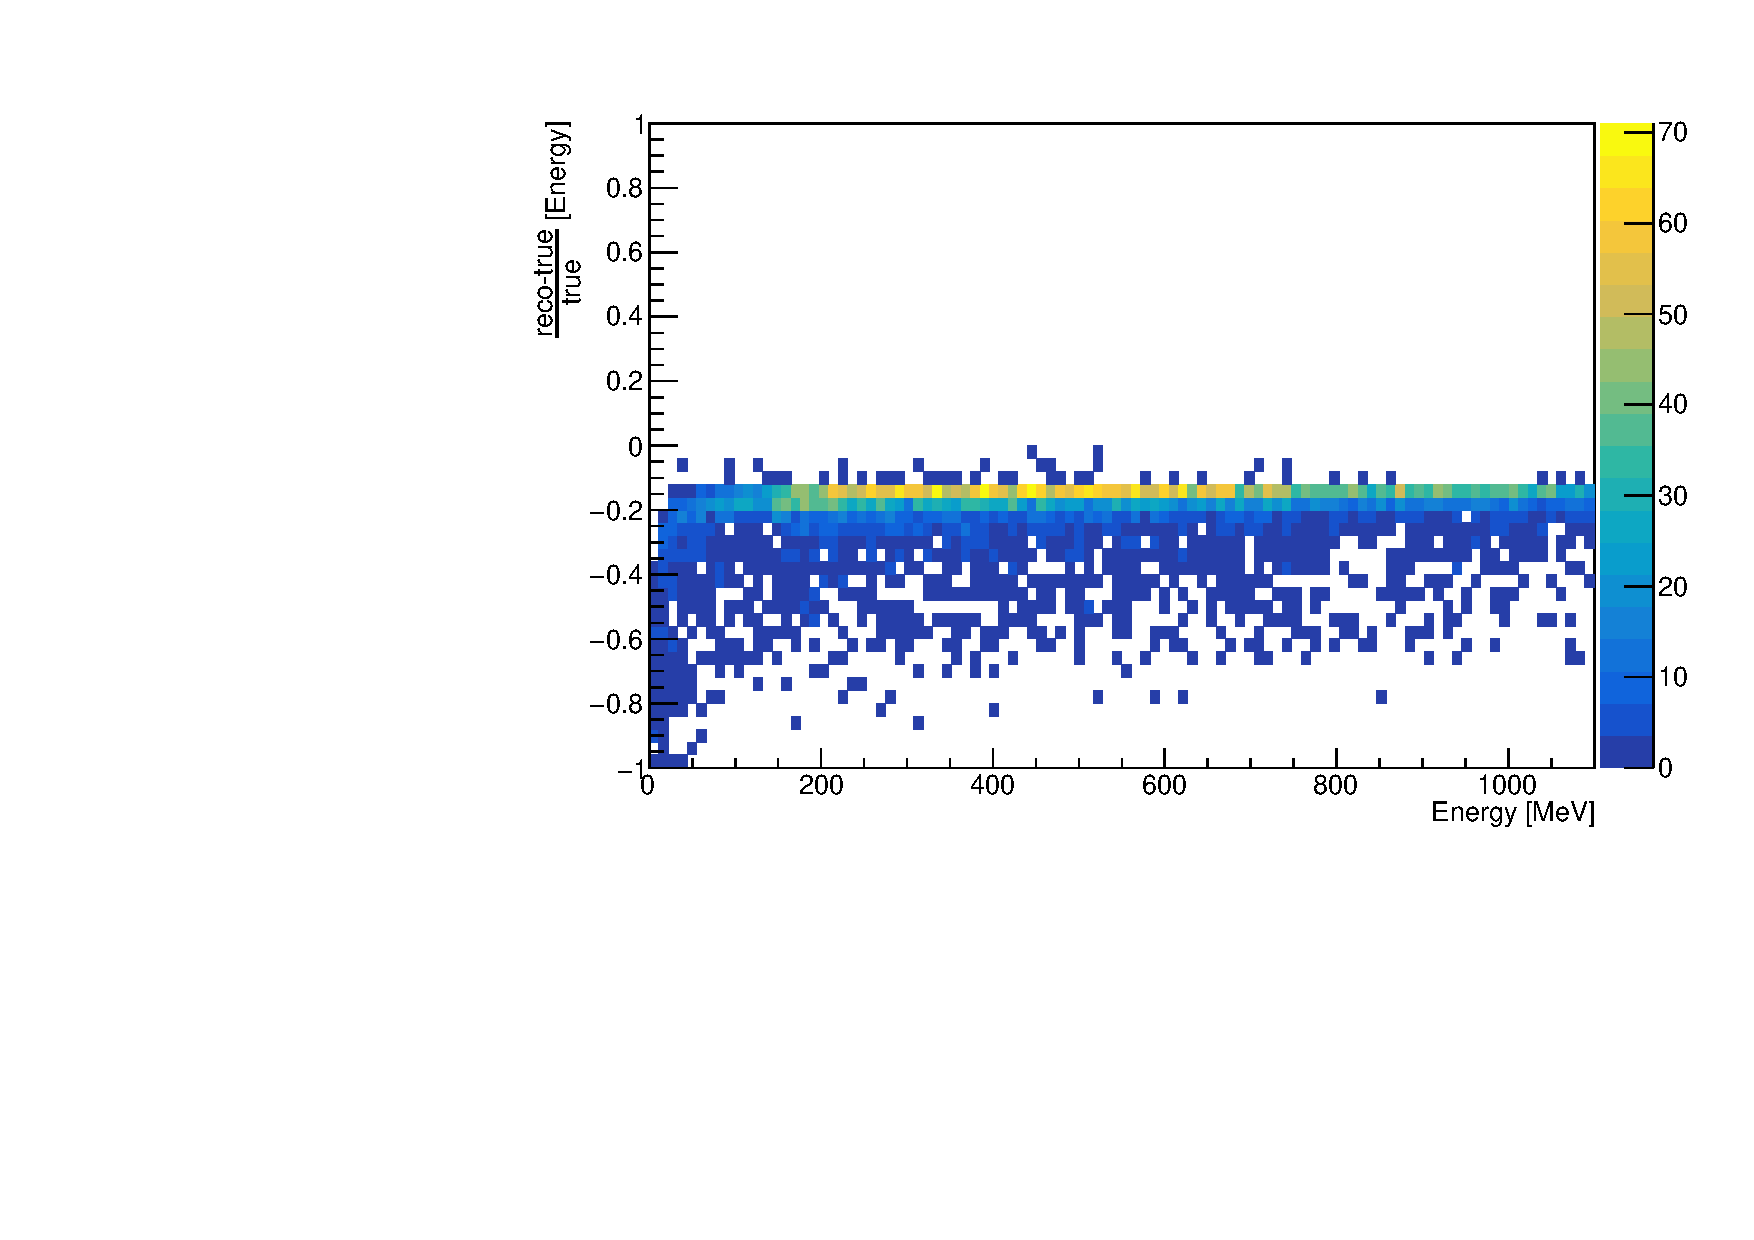
\includegraphics[width = \largefigwidth]{Figures/frac_res_vs_hit_energy_electron_vertex_plane2.pdf}
    \caption{The fractional resolution of the shower energy from an $\electron \pi^+$ vertex sample vs the sum of the true hit energy. Reconstruction performed from the hits collected by plane 2. The resolution is largely consistent across all energies with maybe a minor dip in performance for low energy showers.}
    \label{fig:my_label}
\end{figure}

\begin{figure}
    \centering
    \fbox{Cheated Reco efficiency vs true deposited energy}
    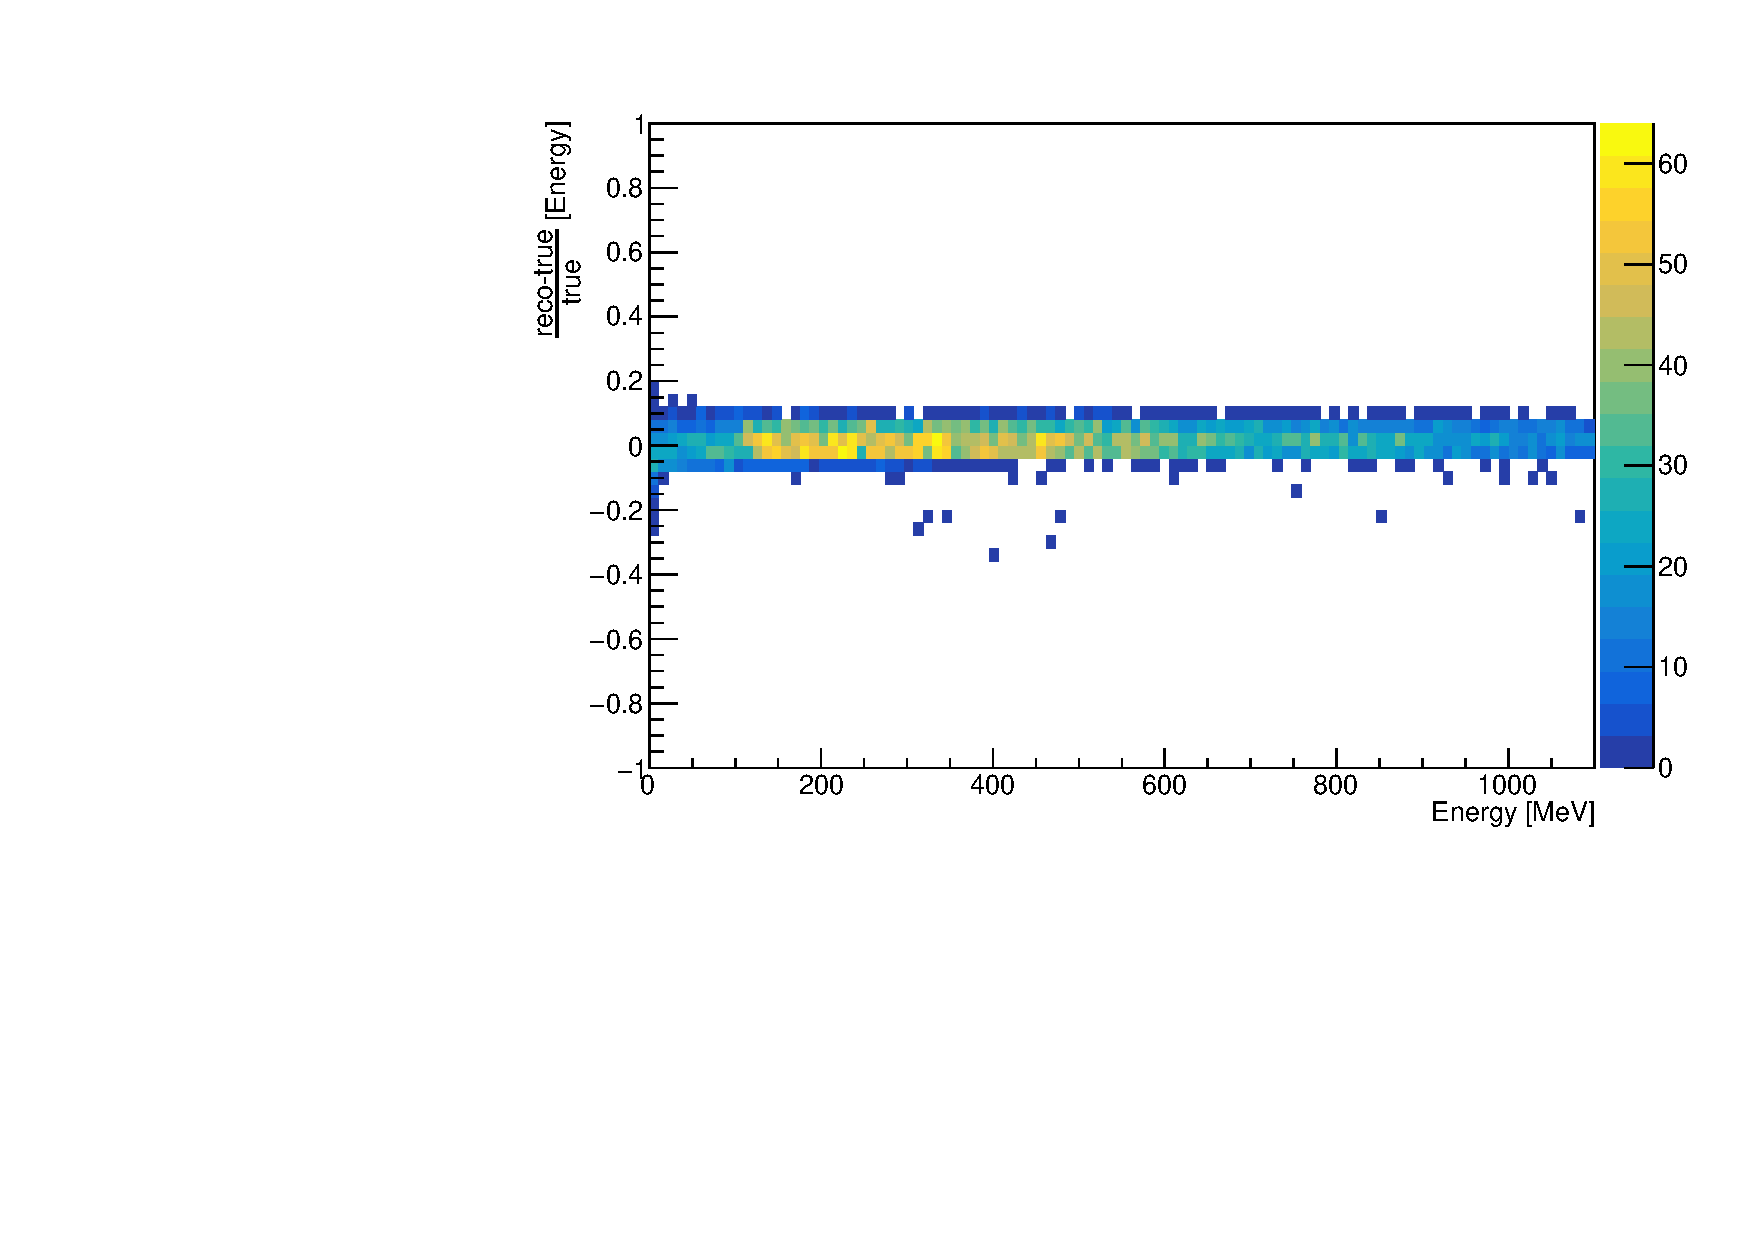
\includegraphics[width = \largefigwidth]{Figures/frac_res_vs_hit_energy_cheating_electron_vertex_plane2.pdf}
    \caption{The fractional resolution of the shower energy from an $\electron \pi^+$ vertex sample vs the sum of the true hit energy. Using cheated pattern recognition with the reconstruction performed from the hits collected by plane 2. The resolution is largely consistent across all energies with maybe a minor dip in performance for low energy showers.}
    \label{fig:my_label}
\end{figure}

\begin{figure}
    \centering
    \fbox{Fractional resolution of \electron $\pi^+$ with lower (no?) hit thresholding.}
    \caption{Caption}
    \label{fig:my_label}
\end{figure}

\begin{figure}
    \centering
    \fbox{Validation with some sort of low energy sample (supernova neutrinos?)}
    \caption{Caption}
    \label{fig:my_label}
\end{figure}




  \chapter{Conclusion}
\label{chap:Conclusion}
  %% To ignore a specific chapter while working on another, making the build faster, comment it out:
  %\input{chap4}
\end{mainmatter}

%% Produce the appendices
\begin{appendices}
  %% The "\appendix" call has already been made in the declaration
%% of the "appendices" environment (see thesis.tex).
\chapter{Pointless extras}
\label{app:Pointless}

\chapter{Some more stuff}

%% Big appendixes should be split off into separate files, just like chapters
%\input{app-myreallybigappendix}

\end{appendices}

%% Produce the un-numbered back matter (e.g. colophon,
%% bibliography, tables of figures etc., index...)
\begin{backmatter}
  %\begin{colophon}
%  This thesis was made in \LaTeXe{} using the ``hepthesis'' class.
%\end{colophon}

%% You're recommended to use the eprint-aware biblio styles which
%% can be obtained from e.g. www.arxiv.org. The file mythesis.bib
%% is derived from the source using the SPIRES Bibtex service.
\bibliographystyle{h-physrev}
\bibliography{mythesis}



%% If you have time and interest to generate a (decent) index,
%% then you've clearly spent more time on the write-up than the 
%% research ;-)
%\printindex

\end{backmatter}




%% Close
\end{document}
